%
% File acl2021.tex
%
%% Based on the style files for EMNLP 2020, which were
%% Based on the style files for ACL 2020, which were
%% Based on the style files for ACL 2018, NAACL 2018/19, which were
%% Based on the style files for ACL-2015, with some improvements
%%  taken from the NAACL-2016 style
%% Based on the style files for ACL-2014, which were, in turn,
%% based on ACL-2013, ACL-2012, ACL-2011, ACL-2010, ACL-IJCNLP-2009,
%% EACL-2009, IJCNLP-2008...
%% Based on the style files for EACL 2006 by 
%%e.agirre@ehu.es or Sergi.Balari@uab.es
%% and that of ACL 08 by Joakim Nivre and Noah Smith

\documentclass[11pt,a4paper]{article}
\usepackage[hyperref]{acl2021}
\usepackage{times}
\usepackage{latexsym}
\usepackage{titlesec}
\usepackage{amsmath}
\usepackage{color,soul}
\setcounter{secnumdepth}{5}
\renewcommand{\UrlFont}{\ttfamily\small}
\usepackage{graphicx}
\graphicspath{{./images/}}
%\usepackage[parfill]{parskip}
\usepackage{booktabs}
\usepackage{array}

% This is not strictly necessary, and may be commented out,
% but it will improve the layout of the manuscript,
% and will typically save some space.
\usepackage{microtype}

\aclfinalcopy % Uncomment this line for the final submission
%\def\aclpaperid{***} %  Enter the acl Paper ID here

%\setlength\titlebox{5cm}
% You can expand the titlebox if you need extra space
% to show all the authors. Please do not make the titlebox
% smaller than 5cm (the original size); we will check this
% in the camera-ready version and ask you to change it back.

\newcommand\BibTeX{B\textsc{ib}\TeX}

\makeatletter
\renewcommand\paragraph{%
    \@startsection{paragraph}{4}{0mm}%
        {-\baselineskip}%
        {.5\baselineskip}%
        {\normalfont\normalsize\bfseries}}
\makeatother

\title{BigGreen at SemEval-2021 Task 1: \\
Lexical Complexity Prediction with Assembly Models}

\author{
  \textbf{Aadil Islam}\normalfont{,} \textbf{Weicheng Ma}\normalfont{, and} \textbf{Soroush Vosoughi}\\
  Department of Computer Science\\
  Dartmouth College\\
  \texttt{\{aadil.islam.21, weicheng.ma.gr, soroush.vosoughi\}@dartmouth.edu}
}

\date{}

\begin{document}
\maketitle

\begin{abstract}
  This paper describes systems submitted by team BigGreen to LCP 2021. We assemble a feature engineering-based model with a deep neural network model founded on BERT. The latter model contextualizes a target expression, given its sentence. While BERT is a strong model overall, the feature engineering-based model helps in extreme cases, eg. separating instances of easy and neutral difficulty. Our handcrafted features comprise a breadth of lexical, semantic, syntactic, and novel phonological measures. Additionally, visualizations of BERT attention maps offer insight into potential features that Transformers models may learn when fine-tuned for lexical complexity prediction. Our ensembled predictions score reasonably well for the single word subtask, and we demonstrate how they can be harnessed to perform well on the multi word expression subtask too.
\end{abstract}

\section{Introduction}

Lexical simplification (LS) is the task of replacing difficult words in a text with simpler alternatives. It is applicable to reading comprehension, where early studies have shown infrequent words to lead to more time a reader spends fixated on it, and that ambiguity in a word's meaning further adds to comprehension time \citep{raynerd86}. Complex word identification (CWI) is believed to be a fundamental step in the automation of lexical simplification \citep{shardlow2014open}. Early techniques for conducting CWI suffer from a lack of robustness, from simplifying all words to then study its efficacy \citep{devlintait}, to applying simple thresholds on discriminative features like word frequency \citep{10.1007/11573067_19}. 

The recent CWI shared task at SemEval-2016 \citep{paetzoldspecia:2016:SemEval1} studied the annotations of 400 non-native speakers on English target words, labeled as either simple or complex. The SemEval-2018 CWI shared task \citep{stajner-EtAl:2018:BEA} extended their study to data across four languages, while also introducing a probabilistic component to the binary classification task. This year's Lexical Complexity Prediction (LCP) shared task \citep{shardlow2020complex} forgoes the treatment of word difficulty as a binary classification task \citep{paetzoldspecia:2016:SemEval1, stajner-EtAl:2018:BEA} and instead measures degree of difficulty on a continuous scale. This choice is intriguing as it mitigates a dilemma with previous approaches of having to treat words extremely close to a decision boundary (suppose a threshold deems a word's difficulty) identically to those that are far away, ie. extremely easy or difficult.

Teams are asked to submit predictions on unlabeled test sets for two subtasks: predicting on single word and multi word expressions (MWEs), respectively. For each subtask, \texttt{BigGreen} presents a machine learning-based approach that fuses the predictions of a feature engineering-based regressor with those of a feature learning-based deep neural network model founded on BERT \citep{DBLP:journals/corr/abs-1810-04805}. Our code is made available on GitHub.\footnote{\url{https://github.com/Aadil101/BigGreen-at-LCP-2021}}

In Sections 2 and 3, we overview related work that inspires our experiments and describe the data used to train \texttt{BigGreen}'s models. For the feature engineering-based model, Section 4 explains six categories of linguistic features experimented with, in addition to feature selection techniques; for the feature learning-based model, we describe its training procedure here. Sections 5 and 6 show how our approaches performed in competition, as well as analysis on worked and what did not.

\section{Related Work}

Previous studies have looked at estimating the readability of a given text, though at the sentence-level rather than word-level. \citet{10.2307/40011226} regresses the number of polysyllabic words in a given lesson against the mean score for students quizzed on information pertaining to the lesson, yielding the SMOG Readability Formula. \citet{10.2307/1473169} offer a list of 768 (later updated to 3,000) words familiar to grade-school students in reading, which they find correlates with the relative difficulty of a given passage. An issue with traditional readability metrics seems to be the loss of generality at the word-level.

\citet{shardlow2013comparison} tries a brute force approach where a simplification algorithm is applied to each word of a given text, deeming a world complex if simplified. However, this suffers from the assumption that a non-complex word does not require further simplification. Also attempted is the assignment of familiarty scores to each word, where a threshold that determining a word's complexity is tuned \citep{shardlow2013comparison}. We avoid thresholding in our study because we find it unnecessary, since raw familiarity scores can be used as features in regression-based tasks. 

Results for the SemEval-2016 task \citep{zampieriEtAl:2017:NLPTEA} suggest vote ensembling predictions of the best performing models as an effective strategy, while several top-performing models \citep{paetzoldspecia2016sv000gg, ronzanoetal2016taln, mukherjeeetal2016ju} appear to use linguistic information beyond just word frequency. Namely, these include lexical, semantic, syntactic, and psycholinguistic features. These findings inspire our use of ensemble techniques, as well us our consideration of phonological features as a point of research. Results from SemEval-2018 show feature engineering-based models outperforming deep learning-based counterparts, despite the latter having generally better performances since SemEval-2016.

\section{Data}

\subsection{CompLex Dataset}

\begin{table}
  \centering
  \begin{tabular}{l|l|r|r|r}
    \toprule
    \centering
    Corpus & Subtask & Train &  Trial &  Test \\
    \midrule
    Bible & Single Word &   2574 &    143 &   283 \\
            & Multi Word &    505 &     29 &    66 \\
    Biomed & Single Word &   2576 &    135 &   289 \\
            & Multi Word &    514 &     33 &    53 \\
    Europarl & Single Word &   2512 &    143 &   345 \\
            & Multi Word &    498 &     37 &    65 \\
    \midrule
    Total & Single Word & 7662 & 421 & 917 \\
          & Multi Word &    1517 &     99 &    184 \\
    \bottomrule
  \end{tabular}
  \caption{\label{tab:datasets} LCP train, trial, and test sets.}
\end{table}

\citet{shardlow2020complex} present CompLex, a novel dataset in which target expressions (single words or MWEs) are assigned a continuous label denoting their lexical complexity. Each label falls in range 0-1, a (normalized) average score given by employed crowd workers who report an expression's difficulty on a 5-point Likert scale. We define a sample's \textit{class} as the bin to which its complexity label belongs (bins corresponding to Likert points). Target expressions in CompLex have 0.395 average complexity and 0.115 standard deviation, reflecting an imbalance in favor of class 2 and 3 samples. 

\begin{table}
  \centering
  \begin{tabular}{l|l|l}
    \toprule
    Corpus & Subtask & Sample \\
    \bottomrule
  \end{tabular}
  \caption{\label{tab:samples} This table will show examples of samples from the single word and MWE train sets.}
\end{table}

Each target expression is accompanied by the sentence it was extracted from, where certain target words appear multiple times in the dataset (in different contexts). A target expression is drawn from one of three corpora (Bible, Biomed, and Europarl) in an effort to motivate study of domain-specific linguistic features. A summary of train, trial,\footnote{In our study we avoid the trial set as we find it to be less representative of the training data, opting instead for training set cross-validation, stratified by corpus and complexity label.} and test set samples is given in Table \ref{tab:datasets}.

\subsection{External Datasets}

We use four additional corpora to extract term frequency-based features for training our feature engineering-based model:

\begin{itemize}
  \item \textbf{English Gigaword Fifth Edition} (Gigaword): this comprises articles from seven prominent international English newswires, acquired by the Linguistic Data Consortium (LDC) \citep{gigaword}.
  \item \textbf{Google Books Ngrams, version 2} (GBND): this is used to count occurences of phrases across a corpus of books, accessed via the PhraseFinder API \citep{phrasefinder}.
  \item \textbf{British National Corpus, version 3} (BNC): this is a 100 million word collection of British written and spoken English \citep{BNC}.
  \item \textbf{SUBTLEXus}: this consists of American English subtitles totaling 51 million in words, whose creators offer a multitude of word frequency lists for \citep{Brysbaert2009MovingBK}.
\end{itemize}

\section{BigGreen Systems \& Approaches}

In this section, we overview information fed to the feature engineering-based system, as well as training techniques for the feature learning-based model. We also describe methods for ensembling their predictions for each subtask. Note that the fitted models for the single word subtask are then harnessed for the MWE subtask.

\subsection{Feature Engineering-based System}

\subsubsection{Feature Extraction}

We aim to capture a breadth of information pertaining to the target word and its context. The majority of features appear to follow heavily right-skewed distributions, which we attribute to Zipf's law manifesting over our plethora of word frequency-based measures. This prompts us to consider both logged and unlogged versions of features. For the MWE subtask, features are extracted independently for the head and tail words, with they and their \textit{sums} being included in the final feature set.

\paragraph{Lexical Features}

These are features based on lexical information about the target word:

\begin{itemize}
  \item \textbf{Word length}: the length of the target word.
  \item \textbf{Number of syllables}: the number of syllables in the target word, computed using the Syllables library\footnote{\url{https://github.com/prosegrinder/python-syllables}}.
  \item \textbf{Is acronym}: whether the target word is a sequence of capital letters.
\end{itemize}
  
\paragraph{Semantic Features}

These features capture the target word's meaning:

\begin{itemize}
  \item \textbf{WordNet features}: the number of hyponyms and hypernyms associated with the target word in WordNet \citep{Fellbaum:2005}.
  \item \textbf{GloVe word embeddings}: we extract 300-dimension embeddings pre-trained on Wikipedia-2014 and Gigaword \citep{pennington2014glove} for each (lowercased) target word. 
  \item \textbf{ELMo word embeddings}: we extract 1024-dimension embeddings pre-trained on the One Billion Word Benchmark corpus \citep{Peters:2018} for each target word. Observe that these are \textit{contextualized} embeddings, unlike the aforementioned GloVe embeddings. 
  \item \textbf{GloVe context embeddings}: we obtain the average 300-dimension GloVe word embedding over each token in the given sentence.
  \item \textbf{InferSent context embeddings}: we obtain 4096-dimension InferSent embeddings \citep{conneau-EtAl:2017:EMNLP2017} for each sentence.
\end{itemize}

\paragraph{Phonetic Features}

These features compute the likelihood that consecutive soundable segments comprising the target word would arise in the English language. Before extraction, we empirically estimate the ground truth transition probabilities between any two units (phonemes or characters) in the English language using the Gigaword corpus. 

\begin{itemize}
  \item \textbf{Phoneme transition probability}: we consider the minimum, maximum, average, and standard deviation over the set of estimated transition probabilities of the target word's phoneme bigrams.
  \item \textbf{Character transition probability}: analogous to the extraction procedure for phoneme transition probability, but over \textit{character} bigrams.
\end{itemize}

\paragraph{Word Frequency and N-gram}

These features are expressly included due to their expected importance as predictors, as indicated by \citet{zampieriEtAl:2017:NLPTEA}.

Gigaword serves as the primary corpus from which we extract word frequency measurements pertaining to the target word. These include term frequency (for both lemmatized and unlemmatized target word), the summed frequency of the target word's byte pair encodings (BPEs), and the summed frequencies of bigrams and trigrams containing the target word. We complement these features with their IDF-based analogues, and count the number of out-of-vocab words in a sentence.

We also incorporate the GBND, BNC, and SUBTLEXus corpora by extracting secondary word frequency, bigram, and trigram measures. 

\paragraph{Syntactic Features}

These are features that assess the syntactic structure of the sentence in relation to the target word. Certain features rely on the construction of a constituency parse tree for the target word's context, which we obtain using a Stanford CoreNLP pipeline \citep{manning-EtAl:2014:P14-5}.

\begin{itemize}
  \item \textbf{Part of speech (POS)}: the part of speech tag predicted using the NLTK Python library's \texttt{pos\_tag} function \citep{Loper02nltk:the}.
  \item \textbf{Depth of parse tree}: this measures the height of the parse tree.
  \item \textbf{Depth of target word}: this measures the distance in number of edges between the target word and the parse tree's root node.
  \item \textbf{Is proper}: whether the target word is a proper noun/adjective, detected using capitalization.
\end{itemize}

\paragraph{Readability Metrics}

These comprise a variety of readability tests applied on the target word's context, using low-level traits such as total word count and total syllable count. Interestingly, certain readability tests count the \textit{difficult} words in a given sentence by assuming rules as to what makes a given word \textit{complex} (eg. the Dale-Chall readability formula \citep{10.2307/1473169} checks a given word against a predetermined list of familiar words). This inspires us to conduct multiple readabililty tests via the Textstat library\footnote{\url{https://github.com/shivam5992/textstat}}, including Flesch-Kincaid grade level, Gunning Fog index, and SMOG index.

\subsubsection{Feature Selection}

For the single word subtask, we try selecting features using a combination of filter and wrapper methods. Our intention is to leverage successful techniques in the MWE subtask too, where we extract head-specific and tail-specific features.

\paragraph{Filter Methods}

\textbf{Variance}: Features are screened by variance of their distributions, with those lower than 0.01 deemed quasi-constant and removed. 

\textbf{Mutual Information}: Features are ranked by their mutual dependence with lexical complexity, and the top-$k$ features are selected. We tune $k$ by evaluating linear regression models fitted on the top-$k$ features, settling on $k=300$. See Figure \ref{fig:mi}.

\begin{figure}
  \centering
  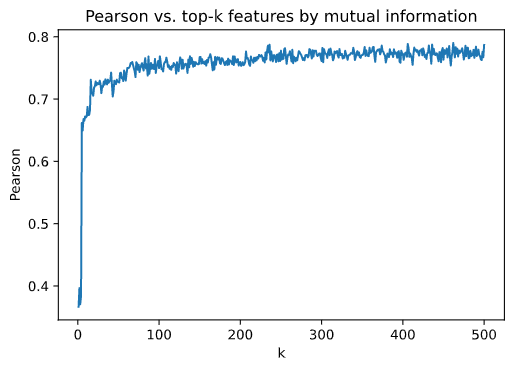
\includegraphics[scale=0.4]{mi.png}
  \caption{\label{fig:mi} Performances of LR fitted on top-k features by mutual information (with 5-fold cross-validation).}
\end{figure}

\textbf{Variance Inflation Factor (VIF)}: VIF is computed for each feature to measure contributed multicollinearity. Note that we omit this particular filter method for the submitted model, for the sake of optimizing Pearson correlation.

\paragraph{Wrapper Methods}

\textbf{Forward Feature Selection (FFS)}: Beginning with an empty feature set, each subsequent iteration appends a new feature to the existing feature set that offers the best Pearson correlation. We end the algorithm when the last added feature fails to sufficiently improve Pearson correlation.

\paragraph{Embedded Methods}

\textbf{Lasso \& Elastic Nets}: We consider these linear models during the subsequent training phase, which use L1 and L1/L2 regularization, respectively, to shrink regression coefficients of lesser important features \textit{during} fitting. Lasso \citep{Tibshirani.x} is intruiging due to its ability to reduce the high dimensionality of our feature set (relative to training set size) during fitting. Elastic Net \citep{10.2307/3647580} may succeed particularly in the presence of highly intercorrelated features.

\subsubsection{Training}

Prior to training, we standardize all features to have approximately zero mean and unit variance. For the single word subtask, we fit Linear Regression, Lasso Regression, Elastic Net Regression, Support Vector Regression (with linear kernel),  Support Vector Regression (with radial basis function kernel), K-Nearest Neighbors Regression, and XGBoost Regression models. 

After identifying the best performing model in terms of Pearson correlation, we mitigate the imbalanced nature of the target variable, ie. the multitude of class-1,2,3 samples and relative lack of class-4,5 samples. We devise a sister version of our top-performing model, fit upon a \textit{reduced} training set containing fewer class-1,2,3 samples. We tune the exact percentages removed from each class by performing cross-validation on the training set.

\subsection{System based on Feature Learning and Transfer Learning}

We hypothesize that lexical complexity draws on the target word's relationship to its context. However, our handcrafted feature set relies heavily upon target word-specific features. Beyond N-gram and syntactic features, this results in a cursory analysis of context encapsulating the target word. We seek an alternative approach for feature learning using deep learning approaches.

\subsubsection{Architecture}

LSTM-based approaches have been used to model the contexts of target words in previous works \citep{hartmanndossantos2018nilc, dehertogtack2018deep}. However, an issue with a single LSTM is that it is capable of reading tokens of an input sentence sequentially only in a single direction. It inspires us to try a Transformer-based approach \citep{DBLP:journals/corr/VaswaniSPUJGKP17}, model architecures capable of processing sentences as a whole (instead of word-by-word) by applying \textit{attention} mechanisms over sentences. Attention weights are useful as they can be interpreted as learned relationships between words in a given sentence. BERT \citep{DBLP:journals/corr/abs-1810-04805} is one such language representation model used for a variety of natual language understanding (NLU) tasks.

Multi-Task Deep Neural Network (MT-DNN) proposed by \citet{liuetal2019multitask} offers state-of-the-art results for a variety of NLU tasks by incorporating benefits of both multi-task learning and language model-pretraining. MT-DNN initializes its shared text encoding layers using a pre-trained BERT model, whose later layers we may fine-tune.

We initialize MT-DNN with the BERT base model (cased), and fine-tune the model for 5 epochs, leaving any hyperparameters to their defaults.

\subsubsection{Input Layer}

Data is fed to the model's input layer in \textit{PremiseAndOneHypothesis} format, where the premise and hypothesis are sentence and target word (or MWE), respectively. The data is then tokenized by a BERT Tokenizer, backed by the HuggingFace tokenizers library \citep{wolf_etal_2020_transformers}.

\subsubsection{Output Layer}

The fine-tuned model's output layer returns the predicted lexical complexity for a given target word/expression. We are particularly interested in interpreting the model's attention maps because, as the work of \citep{DBLP:journals/corr/abs-1906-04341} illustrates, it may provide insight into relevant linguistic features learned by a Transformer-based model.

\subsection{Ensembling}

To combine the 2 sets of predictions obtained from our best performing feature engineering-based regression model (from fitting on the \textit{full} and \textit{reduced} training sets, respectively), we first default to using the \textit{full} predictions. We then tune a threshold, where predictions higher than the threshold (ie. likely of class-4,5 samples) are overwritten with their \textit{reduced} predictions. Lastly, we compute a weighted average ensemble of these predictions with those of our MT-DNN model to obtain a final set of single word subtask predictions. 

For the MWE subtask, we harness the fitted feature engineering and feature learning-based models from the single word subtask by predicting the lexical complexities for the head and tail words each. We then compute a weighted average ensemble of these predicted complexities \textit{and} the predictions of the MT-DNN model trained on MWE.

\section{Results}

\begin{table*}[t]
  \centering
  \begin{tabular}{lcccc}
  \hline \textbf{Model} & \textbf{Pearson} & \textbf{Rank} & \textbf{Spearman} & \textbf{MAE} \\ \hline
  Linear Regression	& 0.7347 & - &	0.6993 &	0.0669 \\
  Forward Feature Selection (FFS)	& 0.7313 & - &	0.7053 & 0.0671 \\
  Lasso (alpha=0.0001) &	0.7352 & - &	0.7042 & 	0.0667 \\
  ElasticNet (alpha=0.001) &	0.7396 & - &	0.7122 &	0.0662 \\
  SVM (kernel=linear, C=0.001) &	0.7254 & - &	0.6970 &	0.0678 \\
  SVM (kernel=rbf, C=1, gamma=0.001) &	0.7392 & - &	0.7066 &	0.0668 \\
  KNN (k=20, weights=distance) &	0.7156 & -	& 0.6914 &	0.0710 \\
  \hline
  XGBoost (\textit{full}) &	0.7589 & - &	0.7220 &	0.0645 \\
  XGBoost (\textit{reduced}) &	0.7456 & - &	0.7157 &	0.0751 \\
  XGBoost (\textit{full}+\textit{reduced}) & 0.7576 & - & 0.7220 & 0.0646 \\
  MT-DNN & 0.7484 & -	& 0.7044 & 0.0664 \\
  Ensemble (submission) & 0.7749 & 8 of 54 & 0.7294 & 0.0629 \\
  \hline
  Best competition results & 0.7886 & & 0.7425 & 0.0609 \\ 
  \hline
  \end{tabular}
  \caption{\label{tab:single-word-results} Test set results for single word subtask. }
\end{table*}

\begin{table*}[t]
  \centering
  \begin{tabular}{lcccc}
  \hline \textbf{Model} & \textbf{Pearson} & \textbf{Rank} & \textbf{Spearman} & \textbf{MAE} \\ \hline
  Head predicted complexity & 0.7164 & - & 0.7305 & 0.1281 \\
  Tail predicted complexity & 0.7188 & - & 0.7416 & 0.1306 \\
  MT-DNN & 0.7890 & - & 0.7649 & 0.0766 \\
  Ensemble (post-competition) & 0.8290 & *14 of 37 & 0.8120 & 0.0857 \\
  Ensemble (submission) & 0.7898 & 25 of 37 & 0.7769 & 0.0903 \\
  \hline
  Best competition results & 0.8612 & &  0.8548 & 0.0616 \\ 
  \hline
  \end{tabular}
  \caption{\label{tab:multi-word-results} Test set results for the MWE subtask. (* projection)}
\end{table*}

Here, we present the performances of \texttt{BigGreen}'s systems on test sets for the single and MWE subtasks. See Tables \ref{tab:single-word-results} and \ref{tab:multi-word-results}.

\section{Analysis}

\subsection{Performance}

For feature selection, we find success in selecting the top-300 features by mutual information \textit{and} removing quasi-constant features. The pruned feature set is passed to both our wrapper/embedded methods and a variety of regressors for model comparison, where we find an XGBoost regressor \citep{DBLP:journals/corr/ChenG16} (with hyperparameters tuned using grid search) to excel consistently for the single word subtask. Performances are shown in Table \ref{tab:single-word-results}, where we rank in the top 15\% by Pearson. 

For the MWE subtask, performances are reported in Table \ref{tab:multi-word-results}. Note that for this subtask our submitted predictions differ from our post-competition predictions. We \textit{previously} used a training procedure resembling that for the single word subtask: (1) filter methods for feature selection, (2) XGBoost for regression, and (3) ensembling with MT-DNN. We hypothesize that the fewer number of training samples available for the MWE subtask contributed to the previous procedure's lackluster performance. This inspired us to incorporate the predictive capabilities of our fitted single word subtask models, yielding superior post-competition results.

\subsection{Feature Contribution}

\begin{figure}
  \centering
  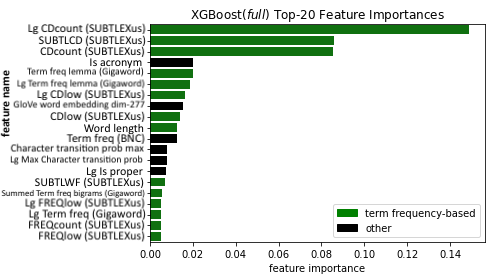
\includegraphics[scale=0.45]{xgboost_feature_importances.png}
  \captionsetup{justification=centering}
  \caption{\label{fig:xgboost_feature_importance} Feature importances for XGBoost(\textit{full}).}
\end{figure}

In total we consider 110 features, in addition to our multidimensional embedding-based features and all $\log$-transformed features. We inspect the estimated feature importance scores produced by the XGBoost(\textit{full}) model to find that term frequency-based features (eg. unigrams, bigrams, trigrams) are of overwhelming importance (see Figure \ref{fig:xgboost_feature_importance}). This raises concern over whether the MT-DNN model too relies on term frequencies to make \textit{its} predictions, and if not, the linguistic features it may have learned upon fine-tuning. Note that of the remaining features possessing non-zero feature importances, the majority appear to be dimensions of one of target word-based semantic features (ie. GloVe or ELMo embeddings).

\subsection{BERT Attention}

\begin{figure}
  \centering
  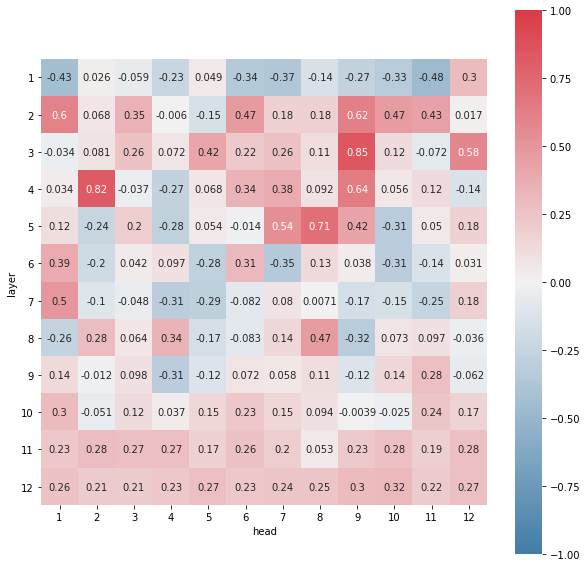
\includegraphics[scale=0.375]{head_correlations_tf.png}
  \captionsetup{justification=centering}
  \caption{\label{fig:head_correlations_tf} Attention head correlation between word frequency and total attention received by word, averaged across 100 random test set samples.}
\end{figure}

\begin{figure}
  \centering
  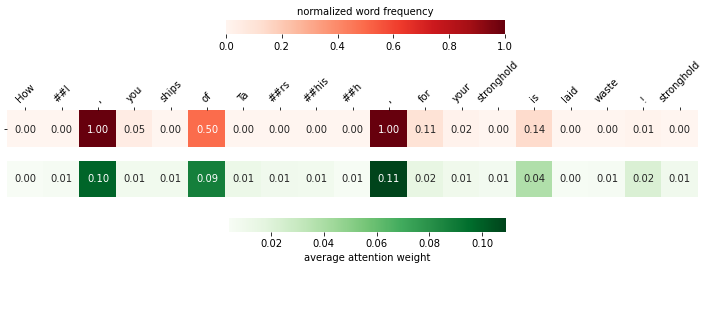
\includegraphics[scale=0.3]{head_3-9_tf_avg.png}
  \captionsetup{justification=centering}
  \caption{\label{fig:head_3-9_tf_avg} Word frequency vs. average head 3-9 attention weight directed to words of a random sample.}
\end{figure}

\begin{figure}
  \centering
  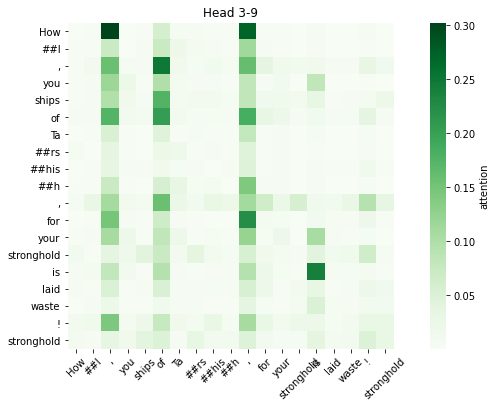
\includegraphics[scale=0.45]{head_3-9.png}
  \captionsetup{justification=centering}
  \caption{\label{fig:head_3-9} Head 3-9 attention map for a random sample.}
\end{figure}

The attention maps of Transformers have in previous works been assessed to demonstrate linguistic phenomena learned by specialized attention heads \citep{1905-09418, 1906-04341} and to measure the relative contribution of each attention head to making task predictions \citep{1905-09418, 1905-10650}. We thereby hope to provide intuition for the MT-DNN model by extracting attention maps from its underlying fine-tuned BERT architecture. For each sample in the single word test set, we extract an attention map from each of the BERT base model's 144 attention heads (ie. 12 heads per 12 layers).

Based on the precedence given to term frequency features by the XGBoost(\textit{full}) model, we hypothesize that for certain attention heads, the degree to which tokens are attended to varies relative to the token's rarity in the lexicon. This follows the findings of \citealp{1905-09418}, who identify heads in which lesser frequent tokens are attended to semi-uniformly by a majority of sentence tokens. 

To test our hypothesis, we estimate for each attention head the Pearson correlation between word frequency and the average attention given to each word in the context.\footnote{We compute attention given to a \textit{word} as the sum of attention given to its constituent byte pair encodings (BPEs). We use the GBND corpus to extract word frequencies from, though any large corpora would suffice.} As illustrated in Figures \ref{fig:head_correlations_tf} and \ref{fig:head_3-9_tf_avg}, we find multiple attention heads appearing to specialize at directing attention towards the most \textit{or} least frequent words (depending on sign of the correlation). Vertical, striated patterns like that in Figure \ref{fig:head_3-9} emerge as a result of attention originating from a spectrum of tokens. The findings seem to affirm the fundamental relevancy of word frequency to lexical complexity prediction, corroborating our intuitions.

\section{Conclusion}

In this paper, we report inspirations for the systems submitted by \texttt{BigGreen} to LCP SharedTask 2021 for their single word and MWE subtasks. We achieve  reasonable performance for the single word subtask by applying simple ensemble methods upon feature engineering-based and feature learning-based models. We see vast potential in future deep learning approaches, while acknowledging the need for strong word frequency-based handcrafted features for the time being. We surpass our submitted results for the MWE subtask, notably through the utilization of the predictive capability of our single word subtask model, and the treatment of MWE complexity as compositional with respect to its tokens.

Avenues for improvement include better data aggregation, as the relative lack of class-4,5 samples hurts Pearson correlation across samples of especially extreme complexity. For instance, an approach may involve synthetic data generation using SMOGN \citep{pmlr-v74-branco17a}. \citet{shardlow2020complex} acknowledge a reader's familiarity with a genre may affect their perceived complexity of a word, however the CompLex dataset lacks details on each annotator's expertise or background, which may offer valuable new insights. Future studies may consider extracting multidimensional embeddings from the later layers of their deep learning models, potentially feeding these embeddings into their feature engineering-based models.

\bibliographystyle{acl_natbib}
\bibliography{anthology,acl2021}

%\appendix

\end{document}
